% Methods

\chapter{Methods} % Main chapter title

\label{Chapter2} % Change X to a consecutive number; for referencing this chapter elsewhere, use \ref{ChapterX}

%----------------------------------------------------------------------------------------
%	SECTION 1
%----------------------------------------------------------------------------------------

\section{System Setup}

\begin{figure}[th]
\captionsetup{justification=raggedright,singlelinecheck=false}
\centering
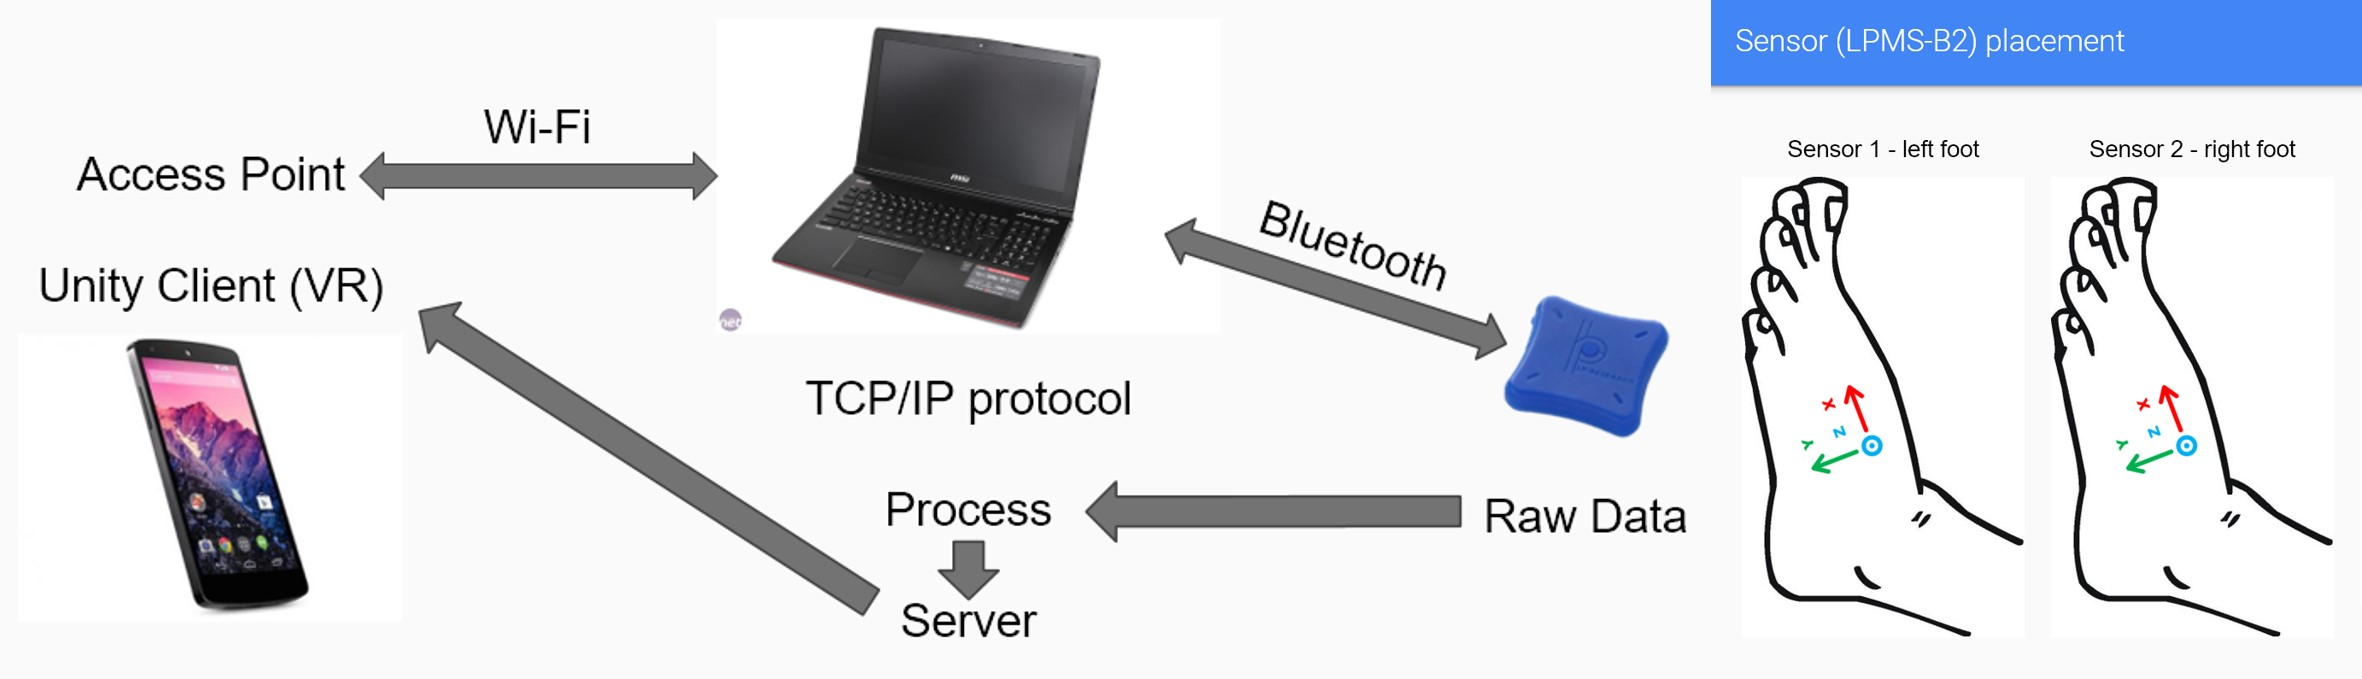
\includegraphics[width=\textwidth,height=\textheight,keepaspectratio]{Figures/system_overview.jpg}
\decoRule
\caption[System overview]{System overview}
\label{fig:system_overview}
\end{figure}
\noindent
System overview is represented in the Figure \ref{fig:system_overview}. System setup consists of a smartphone running Android 6.0 Marshmallow (Nexus 5), a PC running Windows 10 (MSI GE62) and two IMU sensors (LPMS-B2) mounted on each foot as shown in Figure \ref{fig:sensor_module}. For the purpose of this research, IMU sensors are configured to run at 100Hz sampling rate with gyroscope range of 2000$^{\circ}/s$ and accelerometer range of 8G. Though it should be noted that sampling rate of 200Hz is achievable under current configuration. Refer to the datasheet from the manufacturer for detailed specifications. PC acts as a central hub, processing the data received from the IMU sensors and sending the virtual velocity to the smartphone (VR headset). PC and smartphone is connected by Wi-Fi with smartphone providing connection via hotspot and IMU sensors are connected to PC with Bluetooth. Software was developed on Visual Studio 2015 and tested on Unity 5.6.1f1 with sample VR scenes from Udacity. Google Cardboard enables Unity VR projects to run on smartphones running Android 4.4 KitKat or above.  
\\\\
There are three processes - WIP client, Unity client and server. Algorithm presented in this paper is implemented in the WIP client which processes data from IMU sensors and generates virtual velocity. Unity client receives said velocity from the WIP client and displays the virtual environment accordingly. Server maintains a communication session between WIP client and Unity client. WIP client and server runs on the PC and Unity client runs on the smartphone. WIP client is implemented in C++ and the rest is implemented in C\#.

\begin{figure}[th]
\captionsetup{justification=raggedright,singlelinecheck=false}
\centering
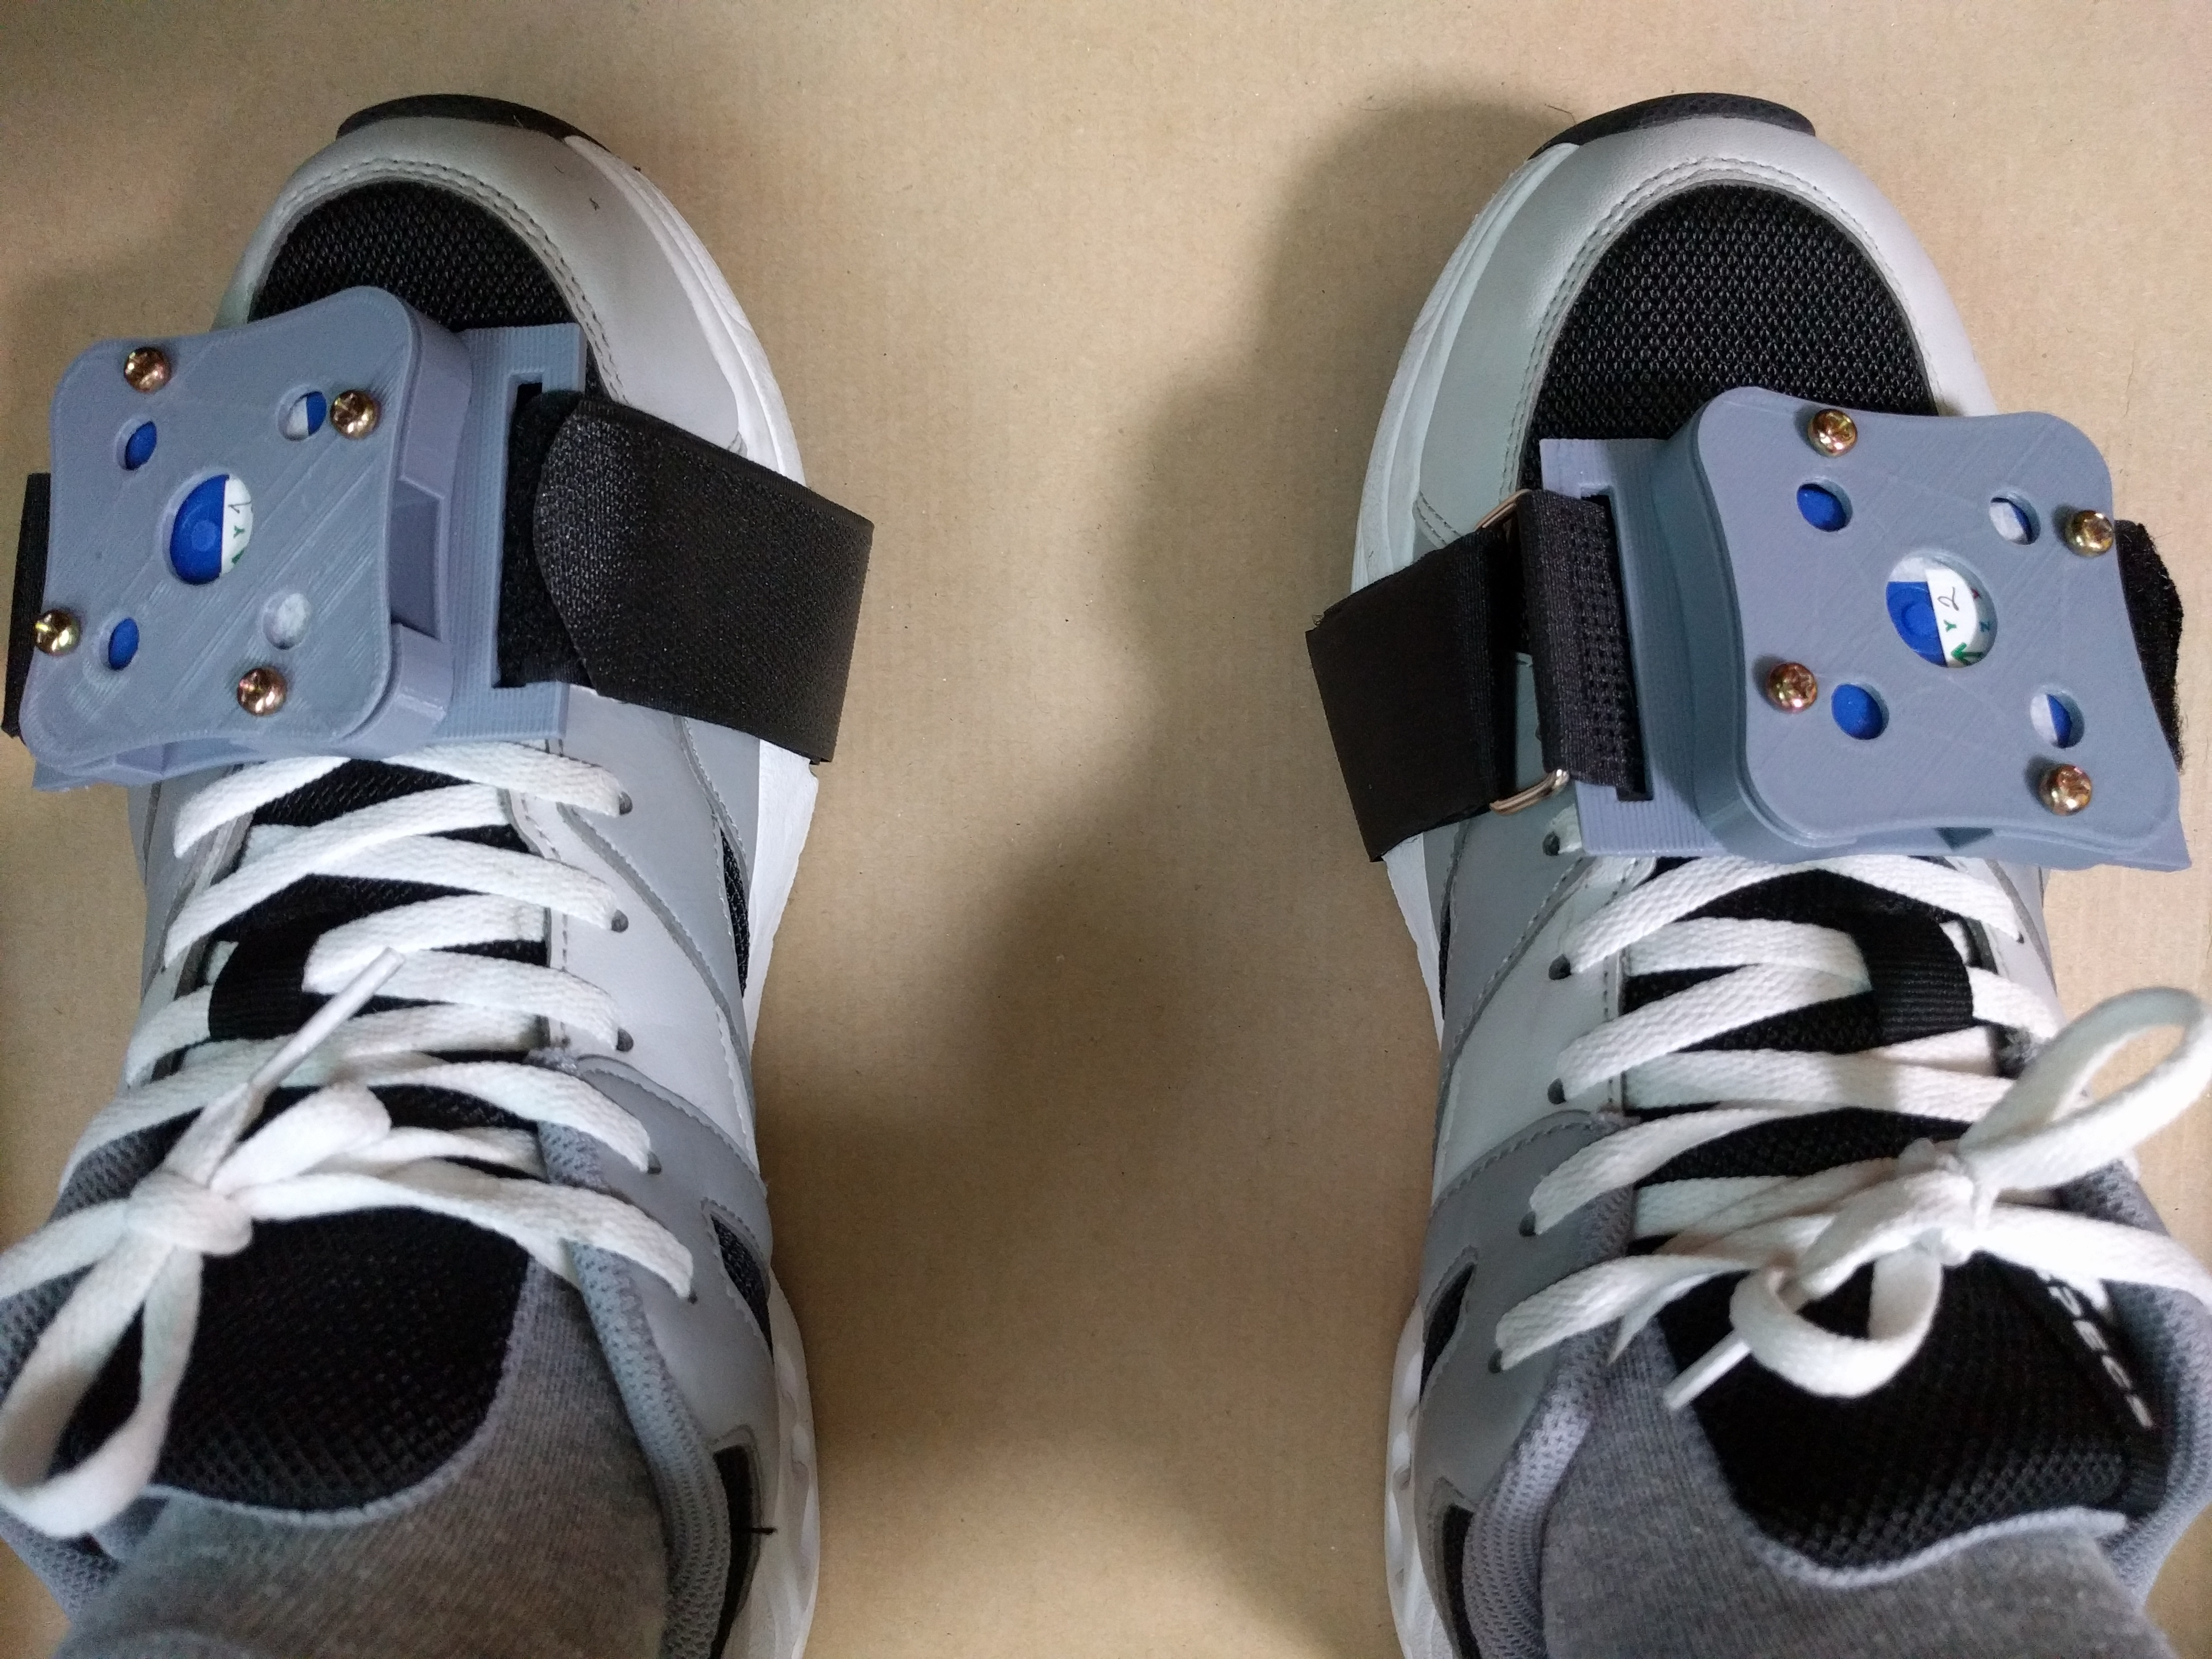
\includegraphics[width=150pt,height=\textheight,keepaspectratio]{Figures/sensor_module.jpg}
\decoRule
\caption[Sensor module with custom brackets]{Sensor module with custom brackets}
\label{fig:sensor_module}
\end{figure}

%----------------------------------------------------------------------------------------
%	SECTION 2
%----------------------------------------------------------------------------------------

\section{Offline Gait Analysis}

Offline gait analysis consist of two parts - event detection and tracking. Gait event detection is implemented with custom FSM (Finite State Machine) with four states and five transitions. Gait tracking borrows from \cite{Kit16} with minor modifications. Gait event detection was not necessary in implementing WIP technique and has been used as a reference only. Kitagawa's algorithm is implemented in the WIP client and executed with 'kita' command (on pre-recorded dataset) or 'calibrate' command (on current recording session).

%-----------------------------------
%	SUBSECTION 1
%-----------------------------------
\subsection{Event Detection}

\begin{figure}[th]
\captionsetup{justification=raggedright,singlelinecheck=false}
\centering
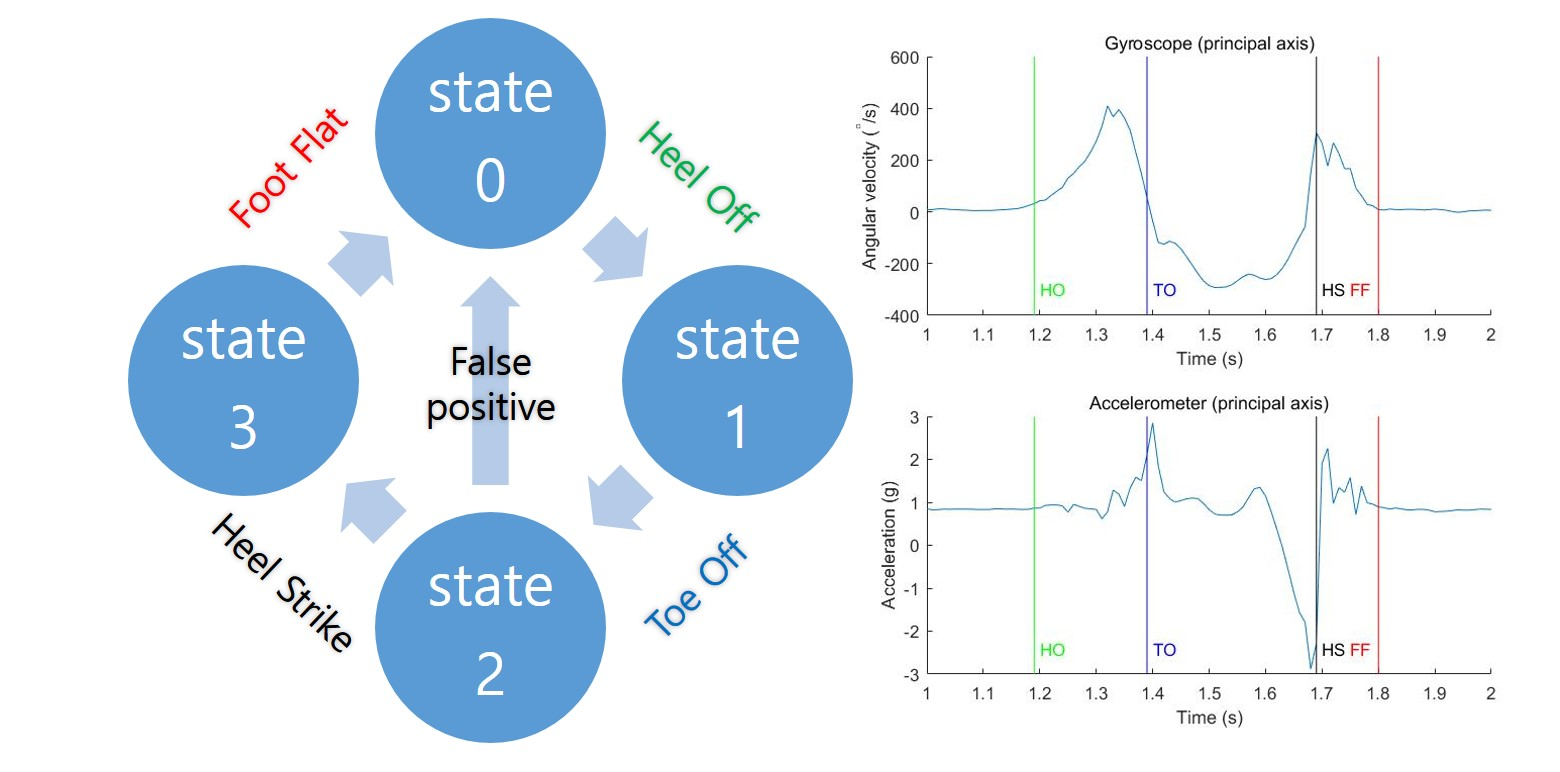
\includegraphics[width=\textwidth,height=\textheight,keepaspectratio]{Figures/gait_event_detection.jpg}
\decoRule
\caption[Gait event detection]{Gait event detection (Right: FSM diagram, Left: gait events superimposed on acceleration and angular velocity along the principal axis)}
\label{fig:gait_event_detection}
\end{figure}
\noindent
Gait event detection relies on gyroscope data only. This is because acceleration can vary depending on sensor placement but angular velocity is independent of sensor placement under the rigid body assumption. Angular velocity along the principal axis, which is defined as the one of the three sensor axes with the largest range of angular velocity, was used to determine the states. This provides better results when compared with using the magnitude of angular velocity - which ensures coordinate invariance - without adding too much complexity. For optimal results it is recommended to roughly align one of the sensor axes to the ankle joint axis. 
\\\\
FSM was devised with functional analysis of the principal axis angular velocity time series (Figure \ref{fig:gait_event_detection}). Initial state (i.e. foot is stationary) is state 0. Transition from state 0 to state 1 occurs when heel-off event is detected. Heel-off event is defined as when the angular velocity exceeds 30$^{\circ}/s$ and is increasing with time. Toe-off event, which is defined as when zero crossing has occurred and the time derivative is less than -2000$^{\circ}/s^{2}$, triggers the transition from state 1 to state 2. Two transitions are defined for state 2. Transition to state 3 occurs when heel-strike is detected. Heel-strike is defined as when zero crossing in the other direction has occurred and the time derivative is greater than 2000$^{\circ}/s^{2}$. Transition to state 0 occurs when there is a false positive and gait is not recognized. This condition is satisfied to be when the angular velocity is greater than zero for certain time steps prior to heel-strike. Foot-flat event, which is defined as when angular velocity is below 10$^{\circ}/s$, triggers the transition from state 3 to state 0. The sign of the principal angular velocity might have to be flipped to match the graph in Figure \ref{fig:gait_event_detection} if the sensor placement does not follow the one shown in Figure \ref{fig:system_overview}.

%-----------------------------------
%	SUBSECTION 2
%-----------------------------------
\subsection{Tracking}

\begin{figure}[th]
\captionsetup{justification=raggedright,singlelinecheck=false}
\centering
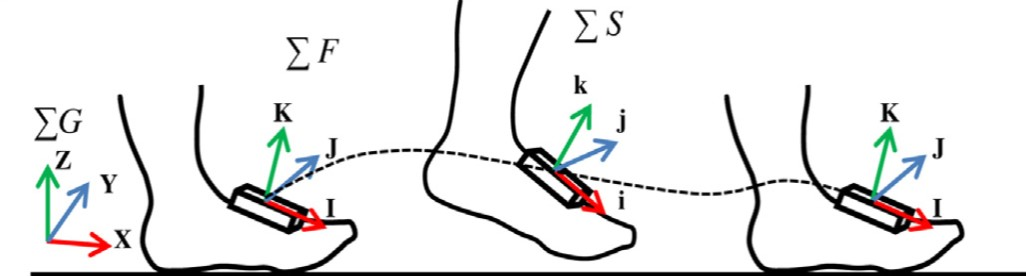
\includegraphics[width=\textwidth,height=\textheight,keepaspectratio]{Figures/kitagawa.jpg}
\decoRule
\caption[Kitagawa's method]{Figure from \cite{Kit16}. Ground frame G is fixed to the ground. Sensor frame S is fixed to the sensor and F is the sensor frame at foot-flat.}
\label{fig:kitagawa}
\end{figure}
\noindent
Gait tracking algorithm follows the method described in \cite{Kit16} but implemented with quaternions instead of rotation matrices for coordinate transformations. Kitagawa's method performs double integration with velocity and position drift correction for accurate gait trajectory tracking. From the gait trajectory, spatio-temporal gait features can be extracted. For detailed description of the algorithm, refer to Kitagawa's paper. A summary is provided below. 
\\\\
1. Find foot-flat and foot-off time with simple thresholding of angular velocity to obtain $T_{0}$ and $T_{f}$.\\
2. Save acceleration $a_{F0}$ (gravity) and orientation quaternion $q^{F}_{G}$ at $T_{0}$ .\\
3. Find linear acceleration in G coordinates between $T_{0}$ and $T_{f}$.\\
\indent
a. Represent raw sensor acceleration in F coordinates ($a_{Ft}$).\\
\indent
b. Subtract $a_{F0}$ to obtain gravity compensated linear acceleration.\\
\indent
c. Represent said value in G coordinates.\\
4. Integrate linear acceleration by time and apply velocity drift correction such that the velocity is zero at $T_{f}$.\\
5. Integrate once more and apply positional drift correction such that the vertical component of position is zero at $T_{f}$.

%----------------------------------------------------------------------------------------
%	SECTION 3
%----------------------------------------------------------------------------------------

\section{Real-time WIP Tracking}

Real-time WIP tracking can be difficult due to the real-time aspect. Unlike offline analysis where the entire time series is available, real-time applications have to work with data up to the current time point. Moreover, system lag and overall latency also becomes an issue for real-time applications. Specifically for tracking WIP in real-time, estimating velocity drift rate which affects the tracking accuracy of the consequent step is crucial. This can be done by taking into account the history of past velocity drift rates with a feedback loop. With the feedback loop in place complications such as ensuring the stability of the system arise.

%-----------------------------------
%	SUBSECTION 1
%-----------------------------------
\subsection{FSM}
%WIP event detection is implemented with BSM (Binary State Machine) which relies on IMU data with simple threshold functions. In order to improve system latency, orientation quaternion relative to foot-flat orientation is decomposed into xy rotation and z rotation components which is then converted into axis-angle representation to be processed with threshold function.

\begin{figure}[th]
\captionsetup{justification=raggedright,singlelinecheck=false}
\centering
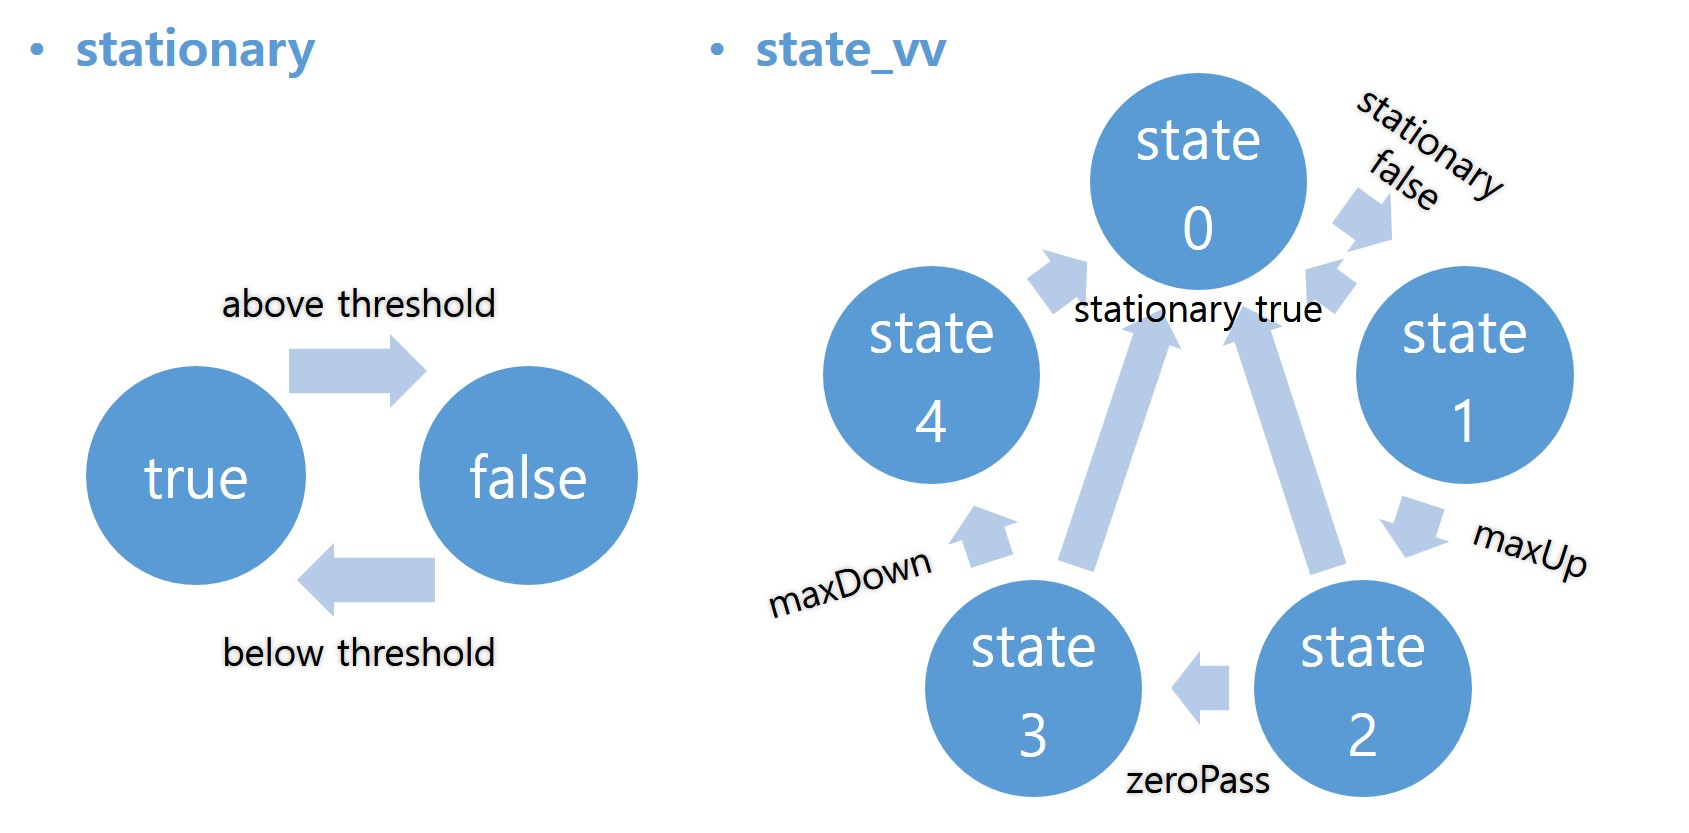
\includegraphics[width=\textwidth,height=\textheight,keepaspectratio]{Figures/WIP_FSM.jpg}
\decoRule
\caption[FSM diagram for WIP motion]{FSM diagram for WIP motion (Left: stationary, Right: state\_vv)}
\label{fig:WIPFSM}
\end{figure}
\noindent
There are two FSMs for real-time WIP motion tracking as shown in Figure \ref{fig:WIPFSM}. FSM for stationary utilizes simple thresholding for state transition. Thresholding is performed on band-pass filtered acceleration and low-pass filtered angular velocity. If the filtered values are under the user configurable thresholds, foot is assumed to be stationary. Through trial and error optimal threshold was set as 0.04G and 30$^{\circ}/s$ for acceleration and angular velocity thresholds, respectively. Band-pass filter for acceleration was implemented as subtracting known offset of 1G (gravity) from raw acceleration magnitude which was then processed with first order digital IIR (Infinite Impulse Response) low-pass filter with a cutoff frequency of 5Hz and a sampling rate of 100Hz.
\\\\
FSM for state\_vv was devised with functional analysis of the vertical component of the foot velocity. Under WIP motion, foot travels up and down resulting in a vertical velocity profile that is sine-like. When foot is stationary, state\_vv is at state 0. Otherwise state\_vv follows a clockwise state transition triggered by events maxUp, zeroPass, maxDown (Figure \ref{fig:WIPFSM}). maxUp event is when foot reaches maximum upwards velocity, followed by zeroPass event when the foot reaches the apex  and heads back down. maxDown event is when foot reaches maximum downwards velocity.

%-----------------------------------
%	SUBSECTION 2
%-----------------------------------
\subsection{Position Tracking}
The basic idea behind real-time WIP position tracking algorithm is similar to Kitagawa's method used for gait tracking. However, the real-time aspect introduces some challenges, particularly with drift correction and lag from application of filters in the FSM. Pseudocode of the algorithm is presented below.
\\\\
1. Represent the raw acceleration measured in sensor frame in ground coordinates and subtract gravity (0, 0, 1)G to obtain gravity compensated linear acceleration $a_{G}$.\\
2. During non-stationary periods integrate velocity drift rate corrected linear acceleration by time to obtain velocity in ground coordinates $v_{G}$.\\
3. Integrate once more during non-stationary periods to obtain position in ground coordinates $x_{G}$. If the vertical component of position falls below zero said component is set to zero. Also, during stationary periods $x_{G}$ is set to zero.\\
4. Let $v_{G}$ at transition from non-stationary to stationary be drift velocity $v_{drift}$ and the duration of the last non-stationary session be $\Delta t$. Then the velocity drift rate is updated by the following equation in feedback form.\\\\
\centerline{$\dot{v}_{drift} = \dot{v}_{drift} + v_{drift}/\Delta t$}
\\\\
When compared with Kitagawa's method there is a minor difference in deriving gravity compensated linear acceleration. This is because the definition of $T_{0}$ is complicated to implement in a real-time fashion. Major difference is in drift correction. With real-time tracking it is impossible to know the exact the value of the velocity drift rate beforehand, thus velocity drift rate from the previous session is assumed as the velocity drift rate. This results in reduced accuracy when compared with Kitagawa's method and is a trade-off for running in real-time.

%----------------------------------------------------------------------------------------
%	SECTION 4
%----------------------------------------------------------------------------------------

\section{Locomotion Generation}

A direct and an indirect approach for locomotion generation scheme has been devised. Direct approach reconstructs horizontal velocity of the foot under normal gait from the vertical position of the foot in WIP motion. Simulated horizontal velocity of each foot is then manipulated to generate locomotion in the virtual environment. This approach is largely inspired by the method described in \cite{Fea08} which derives locomotion from signal processing of heel height. Indirect approach generates locomotion from spatio-temporal parameters extracted from WIP motion such as maximum foot height and non-stationary duration. This approach is more in line with recent research such as \cite{Bru13} and \cite{Tre16}.

\newpage
\subsection{Direct Approach}
Direct approach is based on the simple assumption of the WIP motion. One of the simple ways of modelling ankle trajectory during gait is assuming a cycloid trajectory ($t - sin(t)$, $1 - cos(t)$). Then the time derivative of horizontal and vertical component of the cycloid follow $1 - cos(t)$ and $sin(t)$, respectively. Note that the vertical component of the cycloid trajectory and the horizontal component of the time derivative follow the same profile $1 - cos(t)$. Thus, the horizontal velocity of the foot can be reconstructed from vertical position of the foot with an appropriate scale factor. This scale factor can be determined from the results of offline gait analysis. Assuming one-to-one correspondence between vertical components of walking and WIP motion, it is possible to reconstruct horizontal motion from WIP motion. Aforementioned assumptions have been backed with actual data as shown in Figure \ref{fig:cycloid}. Note that the vertical component of walking is not entirely sine-like which is due to the fact that the sensor was mounted at the dorsum of the foot. With reconstructed horizontal motion for both feet, torso velocity is determined by the average of reconstructed feet speeds.
\\\\
\centerline{$v_{z, walking} = V_{z}sin\Big(\dfrac{2\pi}{T}t\Big)$}
\centerline{$v_{r, walking} = V_{r}\Big[1 - cos\Big(\dfrac{2\pi}{T}t\Big)\Big]$}
\centerline{$p_{z, walking} = \int v_{z, walking}dt = \dfrac{TV_{z}}{2\pi}\Big[1 - cos\Big(\dfrac{2\pi}{T}t\Big)\Big]$}\\\\
\centerline{$scale factor = \dfrac{v_{r, walking}}{p_{z, walking}} = \dfrac{2\pi V_{r}}{TV_{z}}$}

\begin{figure}[th]
\captionsetup{justification=raggedright,singlelinecheck=false}
\centering
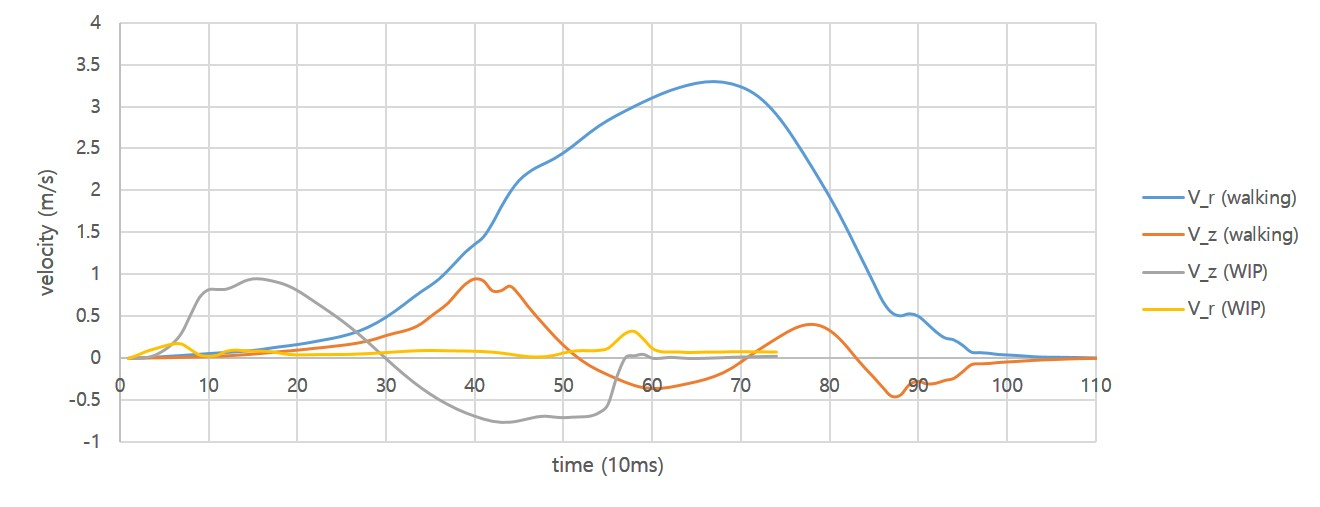
\includegraphics[width=\textwidth,height=\textheight,keepaspectratio]{Figures/cycloid_profile.jpg}
\decoRule
\caption[Sample velocity profile for walking and WIP motion]{Sample velocity profile for walking and WIP motion}
\label{fig:cycloid}
\end{figure}
\noindent
Practical issues arise during implementation. Simple averaging of reconstructed foot motion results in jerkiness. This is due to brief double stance phase causing the motion to abruptly stop midway. Similar issues were discussed by \citep{Fea08} and was mitigated by adopting a low-pass filter to smooth out the locomotion with minor compromise regarding increased stopping latency. In this paper, extra measures were taken to prevent jerkiness and to keep the stopping latency relatively low. When state\_vv is at state 4 ($t_{4}\leq t$), extra padding is applied to prevent speed from falling to zero. The equation is provided below.
\\\\
\indent
$v_{r, reconstructed} = scale factor\times p_{z, WIP}(t)$\indent($t_{1}\leq t\leq t_{4}$)\\
\indent
$v_{r, reconstructed} = 0.5\times scale factor\times (p_{z, WIP}(t) + p_{z, WIP}(t_{4}))$\indent($t_{4}\leq t$)\\
\indent
$v_{locomotion} = 0.5\times(v_{r, reconstructed (left)} + v_{r, reconstructed (right)})$

\subsection{Indirect Approach}
Unlike direct approach, indirect approach does not utilize the entire time series of the foot vertical position. It only requires maximum foot height and non-stationary duration. Higher maximum foot height and shorter non-stationary duration corresponds to faster locomotion. Maximum foot height and non-stationary duration is updated when either one of the foot is at zeroPass (state\_vv transition from state 2 to state 3). The foot is at maximum height at zeroPass and the non-stationary duration is assumed to be double the duration between foot-off and zeroPass. When WIP motion is initiated maximum foot height and non-stationary duration is unknown, thus until one of the feet has reached zeroPass direct approach is used for locomotion. If both feet remains stationary for longer than the user configurable timeout, it is assumed that the user intends to stop. This value will determine the frequency of unintended stops and the stopping latency. In order to distinguish between rotation-in-place and WIP, if maxHeight is under certain threshold (of 0.02-0.03m) speed is set to zero. The equation for indirect approach is presented below.
\\\\
\indent
$v_{locomotion} = scale factor\times maxHeight \times f(WIPPeriod)$,
\\\\
where $f(WIPPeriod)$ is a function that increases as $WIPPeriod$ decreases.

\subsection{Heading}
Locomotion heading can be determined either by user's gaze direction obtained from the headset or by the midway direction of the feet. The latter requires syncing (offset compensation) between the virtual environment frame and the ground frame. Gaze-directed heading is easy to implement as it is provided by the Google Cardboard API. Feet-directed heading needs to be implemented in the WIP client. Pseudocode of said algorithm is provided below.
\\\\
1. Compute relative orientation quaternion to initial orientation quaternion.\\
2. Decompose said quaternion and obtain the two-dimensional direction vector (representing the yaw angle) of both feet.\\
3. Add the direction vector of both feet to obtain midway direction vector.